\documentclass[12pt]{article}
\usepackage[margin=1in]{geometry}
\usepackage[T1]{fontenc}
\usepackage{mathptmx}
\usepackage[parfill]{parskip}
\usepackage{amsmath}
\usepackage{graphicx}
%\usepackage{listings}   % allows lstlisting environment
%\usepackage{moreverb}   % allows listinginput environment
\usepackage{siunitx}
\usepackage{enumerate}
%\usepackage{epstopdf}
%\usepackage{booktabs}
%\usepackage{float}
%\usepackage{enumerate}
%\usepackage{multirow}
%\usepackage{mhchem}
%\usepackage{lscape}
\usepackage{hyperref}
\hypersetup{
    colorlinks=true,
    linkcolor=blue,
    filecolor=magenta,      
    urlcolor=cyan,
}

\newcommand{\horrule}[1]{\rule{\linewidth}{#1}} % Create horizontal rule command with 1 argument of height

\newcommand\mytitle{Evolution 1\\Compsci 458}
\title{\horrule{5pt}\\\vspace{0.4cm}{\bf \mytitle}\\}
\author{Jiawei Zhang, Davis Treybig, Michael Han, and Kevin Do}
\date{\horrule{1pt}}

\begin{document}
\maketitle{}
\section{Summary}
\begin{figure}[h]
\begin{center}
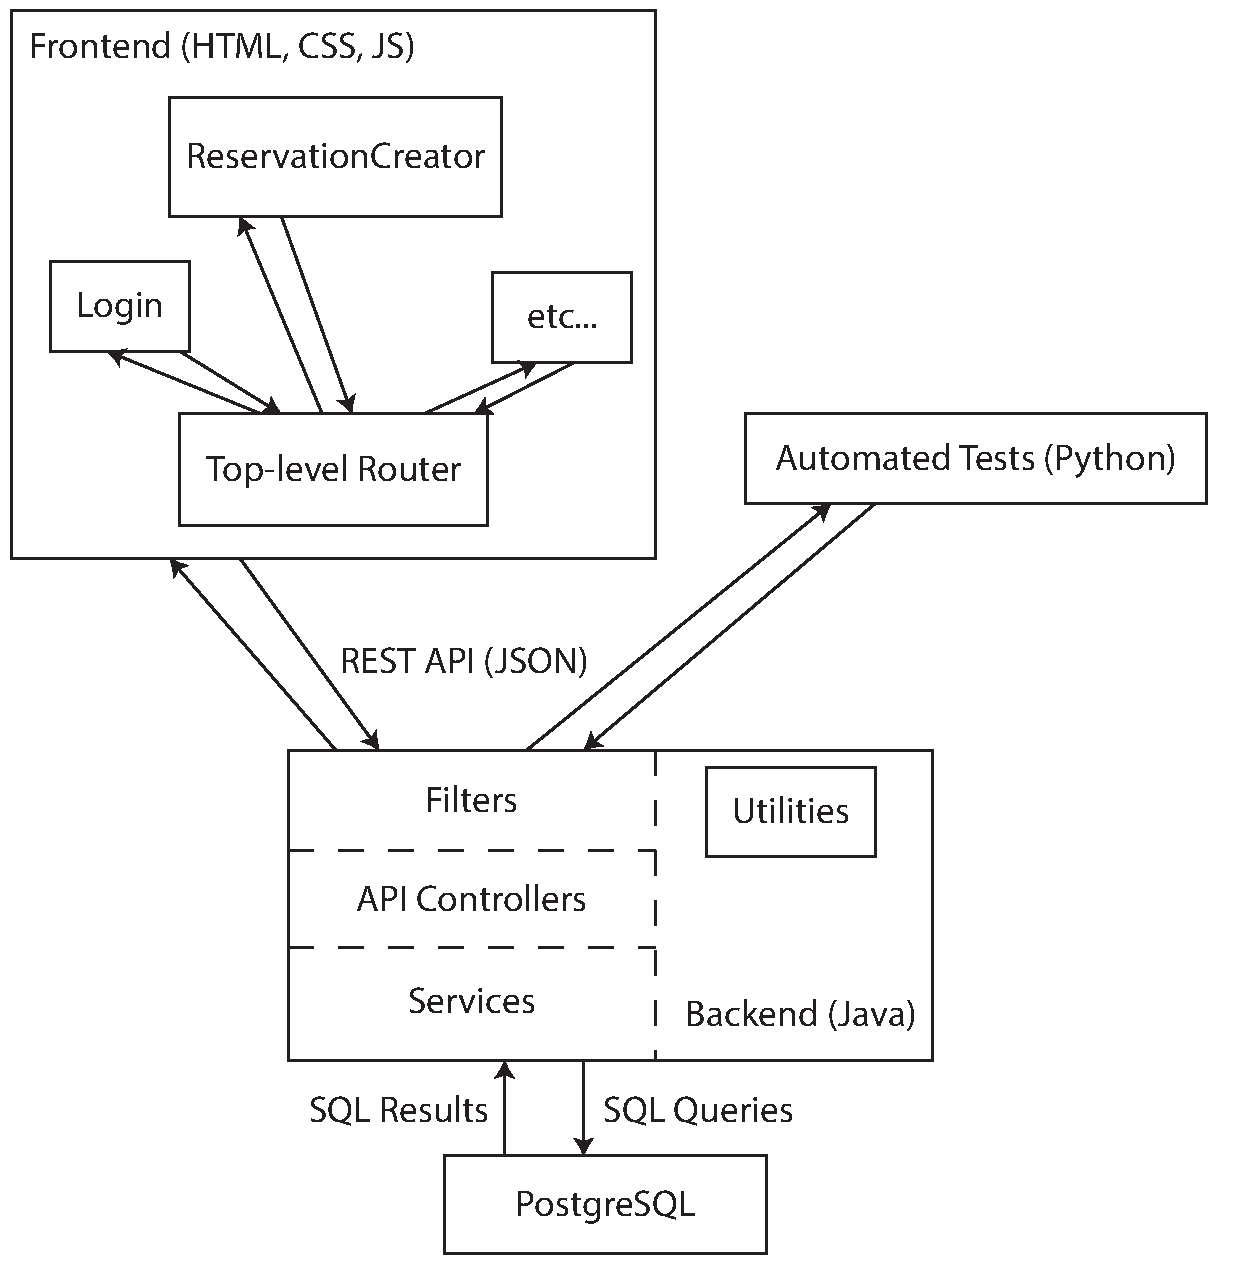
\includegraphics[height=4in]{design_cropped.pdf}
\end{center}
\caption{Diagram of system architecture}
\label{fig:design}
\end{figure}

TODO: Davis

\section{Backend}
The backend consists of the parts of the software system that run on a VPS (Virtual Private Server) using Ubuntu Linux 14.04. Our software uses PostgreSQL 9.5 for persistent data storage and the Java Spring Framework as the container for a Tomcat web server. If the backend were viewed as an MVC (Model-View-Controller), PostgreSQL would be the model while Java Spring both handles the interface of the REST API (view) and the controller that processes requests, communicates with the database, and returns responses. 

\subsection{Java}
The majority of the backend is written in Java. We chose java for a few key reasons:
\begin{enumerate}
    \item It is statically typed. We did not want to deal with the complexity and ambiguity of non-statically typed languages in a group setting where each of us routinely has to read and modify other people's code. 
    \item We found Spring (our Java server framework) to be easy to use and simple to understand, with a huge amount of documentation and support. It is also very powerful and used in many enterprise applications. 
    \item Our whole team is intimately familiar with Java. 
    \item Java has good cross-platform support across all potential server-hosts (particularly in contrast to C\#, another language we considered). Java also has a large standard library and many community libraries, further easing the development process. 
\end{enumerate}

\subsection{Java Spring}
There are a number of open-source application frameworks for Java. Some of the prominent ones that our team looked into are \href{https://www.playframework.com/}{Play}, \href{https://jax-rs-spec.java.net/}{JAX-RS}, \href{http://sparkjava.com}{Spark}, \href{https://spring.io/}{Spring}. Ultimately, we chose to use Spring, for the following reasons:
\begin{enumerate}
    \item Spring is the most oldest, most mature Java web framework. It thus has fantastic documentation and support, as well as a large number of supporting libraries.  These factors make Spring easy to learn, which is vital in the context of a class project where we have to get started developing right away. 
    \item The most common criticism of Spring is that it is too heavy duty and tries to do too much even in simple applications. We personally felt like this was not the case after setting up a sample application.
\end{enumerate}

\subsection{PostgreSQL}
PostgreSQL is an open-source object-relational database management system. 

We chose Postgres over competing relational databases (MySQL) because we were familiar with it from prior experience, and because the small differences between SQL database types are mostly irrelavent for the scope of application we need to develop. 

We chose Postgres over NoSQL databases (MongoDB) because we felt that a relational database could sufficiently store the structured data a resource manager can generate. In addition, we will not be handling live data and we do not need our data to be persistent across evolutions. As such, even if our DB schema changes between evolutions, we will not need to do any sort of schema update to large amounts of existing data. This negates the primary issue of SQL-based databases. Our current DB design can be found in Appendix \ref{appendix:DBDesign}.


\subsection{Encryption}
SSL vs other encryption
spring built in 
keystore using built in java key tool 

jiawei - salt + hash password storage

\subsection{Testing}
For backend testing, we wrote automated tests using Python (Appendix \ref{appendix:backendtest}). We chose not to use Spring's built in testing because it is exceptionally difficult to get working correctly. In contrast, Python scripts are easy to run, simple to understand, and easy to rapidly update and add more tests to. Python's testing framework unittest also has a test discovery function which runs every test with `test' in the function name. This means that we do not have to manually update a separate testing script whenever we add a new test thus improving our design.

Our testing script currently tests only the API contract, and not any internals of the backend. This was done for two reasons. First, the API contract is ultimately the layer that must be working for our front-end application to work, and thus if it works, it is highly likely that there are no significant issues or bugs in our backend code. To some extent, if the application is working from the perspective of the end-user, then it is working correctly. Secondly, it is much harder to test the internals of the back-end, mostly because of our issues using Spring's testing paradigm. That being said, it may be in our best interest to add unit tests in the future if we can figure out how. 

We spent the time to create and maintain an automated testing script because it helps us identify newly introduced bugs much more quickly, and gives each member of the time assurance that they can quickly make changes to the backend without having to thoroughly, manually test after every change. In this way, it speeds up our development cycle. In addition, because automated tests perform the same steps every time, the expected results are consistent which is not always the case with manual testing

\section{REST API}
Communication between the frontend and the backend is done through a REST API with JSON (Appendix \ref{appendix:apispec}). There are several advantages to this approach. RESTful APIs that pass JSON back and forth are well-understood and implemented. The different verbs and endpoints allow for a fairly rich state transfer between the server and the client.

However, there are weaknesses as well. The REST API is based on a request-response paradigm, which means that no data transfer occurs unless it is initiated by the client. In other words, the server has no mechanism to ``push'' updates to the client. Furthermore, JSON is a structured as a tree of values (i.e. there are no pointers or objects). Therefore, relationships between objects have to be hacked together on top of the JSON format (especially many-to-many relationships, which are typically represented in our JSON as subobject relationships).

\section{Frontend}
The frontend consists of the parts of the software system that are transferred to the user's computer and are run in the user's browser. The officially supported browser is the latest version of Google Chrome, but other modern browsers should work as well. We use the third-party libraries React.js, Bootstrap, and JQuery, but React.js has the most implications for the code design.

\subsection{React.js}
The frontend is written in React.js. React is a library written at Facebook for building user interfaces (UIs). The primary paradigm of React is a one-way data flow from ``state'' to a UI. Business logic that wishes to modify the user interface does so by modifying the state. React will then take care of re-rendering the user interface. (React has many performance optimizations, but the general mental model is that the user interface is always an up-to-date rendering of the ``state'').

We chose this framework because we believe that this paradigm is a very natural way of thinking about user interfaces. By thinking of state and how to render this state, we do not worry about performing manual UI updates outside of the React framework. One major advantage of this approach is that we can trivially avoid an inconsistent UI, since the UI always reflects the most recent state. Furthermore, because the UI is a pure function of the state, we can trivially change the way the state is displayed without changing the dataflow plumbing.

\subsection{React components}
Within the React framework, we designed components to express the desired UI in a natural way. At the top level of the HTML body is a Router component. This Router's state includes a route and other state to mediate communication between views. The route is a string that indicates which part of the application the user is in (e.g. ``reservation\_list'').

The Router, depending on its route state, will render one of either a Login, AdminConsole, ReservationList, ReservationCreator, ReservationEditor, ResourceList, ResourceCreator, or ResourceEditor. All of these views are themselves just HTML renders of their state. Each of these subcomponents contains their own state. We considered having a global datastore of resources and reservations, but decided that the simplest way to maintain correctness across views was to simply redownload the data each time.

There is not much to say about the structure of the simple views that are essentially just forms, like Login, AdminConsole, and the creator and editor views. These views maintain their own state (the user input) and send it to the appropriate endpoints when the user submits the form.

The ReservationList and ResourceList views maintain both state about the user's desired display settings (i.e. which tags are required or excluded) and state about what has been downloaded from the server (i.e. which reservations/resources to display). When the user changes display settings, the view then scraps the second state about what has been downloaded, makes a request, and repopulates the state from the JSON response from the server.

\subsection{Testing}
For frontend testing, we decided to write a test plan (Appendix \ref{appendix:frontendtest}) that is intended to be performed manually. Testers can load the application and execute actions that are intended to exercise most of the code paths in the application. This manual testing has the advantage that it has a low upfront cost and it is easy to implement. The disadvantage is that it is slow and takes a lot of human time and energy.

One alternative is to perform automated UI testing. We are aware of two different types automated UI testing: 1) programmatic access to the application and 2) simulation of mouse/keyboard events and screenshots. We decided against 1) because the UI is still in an infantile stage, and the intended DOM changes quite frequently. We decided that programmatically testing for the presence of, say, a certain <div> tag would be prohibitively expensive. We decided against 2) for the same reason that the intended DOM changes quite frequently, but also because we decided that such an approach seemed very fragile.

\section{Member contributions}
Kevin Do designed the initial version of the REST API and implemented the frontend.

Davis Treybig helped write the backend, particularly the Reservation system as well as the Email system. 

\clearpage
\appendix
\section{Backend Test Plan}
\label{appendix:backendtest}
\begin{enumerate}
	\item Authorization Tests
	\begin{enumerate}
		\item Registering a valid user
		\item Registering an invalid user with preexisting email
		\item Registering an invalid user without a password
		\item Logging in as valid user
		\item Logging in with wrong password
		\item Logging in with wrong email, correct username and password
		\item Logging in with wrong username, correct email and password
	\end{enumerate}
	\item Resource Tests
	\begin{enumerate}
		\item Create valid resource with no tags
		\item Create valid resource with tags
		\item Create invalid resource with no name
		\item Create valid resource with no description 
		\item Get resource with valid ID
		\item Get resource with invalid ID
		\item Get resources with valid query
		\item Get resources with query with non existing tags
		\item Put resource with valid ID with all fields updated
		\item Put resource with valid ID no fields updated
		\item Put resource with invalid ID
		\item Delete resource with valid ID
		\item Delete resource with invalid ID
		\item Get resources canDelete with valid ID
		\item Get resources canDelete with invalid ID
	\end{enumerate}
	\item Reservation Tests
	\begin{enumerate}
		\item Create valid reservation with valid user ID
		\item Create valid reservation with invalid user ID
		\item Create reservation with touching time intervals
		\item Create invalid reservation with invalid resource ID
		\item Create invalid reservation with invalid time range
		\item Get reservation with valid ID
		\item Get reservation with invalid ID
		\item Get reservation with valid query with resource and user lists
		\item Get reservation with valid query with valid time range
		\item Get reservation with valid query with invalid time range
		\item Put reservation with valid ID update all fields
		\item Put reservation with valid ID update no fields
		\item Put reservation with invalid ID
		\item Delete reservation with valid ID
		\item Delete reservation with invalid ID
	\end{enumerate}
	\item Tags Tests
	\begin{enumerate}
		\item Get all tags
	\end{enumerate}
	\item User Tests
	\begin{enumerate}
		\item Check only admin can create users
		\item Check that non admin cannot create users
		\item Create invalid user with preexisting username
		\item Create invalid user with preexisting email 
		\item Get user with valid ID
		\item Get user with invalid ID
		\item Put User with invalid ID
		\item Put user not as admin
		\item Delete user with valid ID
		\item Delete user with invalid ID
	\end{enumerate}
\end{enumerate}

\clearpage
\section{Frontend Test Plan}
\label{appendix:frontendtest}
\begin{enumerate}
	\item Login
	\begin{enumerate}
		\item Logging in as the admin works
		\item Logging in as a normal user works
		\item Entering the wrong credentials -> useful message
	\end{enumerate}
	\item Navbar
	\begin{enumerate}
		\item Resources -> resources list
		\item Reservations -> reservations list
		\item Admin console works
		\item Log out works
	\end{enumerate}
	\item Reservations List
	\begin{enumerate}
		\item Start+end can correctly filter reservations shown
		\item Tags can correctly filter reservations shown
		\item Can properly go to the ``New reservation'' view
		\item Can properly go to the ``Edit reservation'' view
		\item Normal user can delete reservations own reservations
		\item Normal user can NOT delete others' reservations
		\item Admin can delete any reservation
	\end{enumerate}
	\item Resources list
	\begin{enumerate}
		\item Tags can correctly filter resources shown
		\item Can properly go to the ``New resource'' view
		\item Normal user can not edit/delete anything
		\item Admin user can edit/delete anything
		\item Deleting a resource with a future reservation shows a warning
	\end{enumerate}
	\item New resource
	\begin{enumerate}
		\item Admin can make new resource
		\item Normal user can't make new resource
		\item Displays error messages when invalid
	\end{enumerate}
	\item New reservation
	\begin{enumerate}
		\item Normal user can make new reservation with their own user ID
		\item Normal user can't make new reservation with another user ID
		\item admin can make new reservation with any user ID
	\end{enumerate}
	\item Admin console
	\begin{enumerate}
		\item Admin can make new user
		\item Normal user can't make new user
	\end{enumerate}
\end{enumerate}

\clearpage
\section{API Specification}
\label{appendix:apispec}
\begin{enumerate}
\item POST /auth/register
Creates an account with specified email and password

Common errors: email taken

Returns a JSON object with is\_error (boolean), error\_msg (possibly empty string)

\item POST /auth/login
Logs into an account with specified email and password

Common errors: invalid email or password

Returns a JSON object with is\_error (boolean), error\_msg (possibly empty string). If is\_error is false, also returns the session token


\item POST /resources
Creates a resource with the specified name, description, and tags, and assigns it a new unique ID

Common errors: empty name

Returns a JSON object with is\_error (boolean), error\_msg (possibly empty string). If is\_error is false, also returns a resource subobject with all the fields that were actually committed (ideally, the same as the values that were passed in)

\item GET /resources/<ID>
Returns a JSON object with is\_error (boolean) and error\_msg (possibly empty string)

Common errors: Resource with the specified ID does not exist

If is\_error is false, also returns a ``resource'' subobject with all the fields of the resource with the supplied ID

\item GET /resources/
Runs the specified query on the set of all resources and returns those that match

Queries are specified by a URL parameters with a ``required\_tags'' object (list of strings) and ``excluded\_tags'' specifying the tags that the resources in the search results should all have

Returns a JSON object with is\_error (boolean) and error\_msg (possibly empty string)

If is\_error is false, also returns a ``resources'' subobject, a list of resources (including ID and all fields) that match the query

\item PUT /resources/<ID>
Updates a resource with the supplied ID. Only changes the supplied fields and leaves the rest alone

Returns a JSON object with is\_error (boolean), error\_msg (possibly empty string). If is\_error is false, also returns a resource subobject with all the fields that were actually committed (ideally, the same as the values that were passed in)

\item DELETE /resources/<ID>
Deletes the resource with the given ID, if it exists, AND deletes all associated reservations

Common error: resource with the specified ID does not exist

Returns a JSON object with is\_error (boolean) and error\_msg (possibly empty string)

\item POST /reservations
Creates a reservation with data specified by the payload's ``resource\_id'' (int), ``start\_timestamp'' (string), ``user\_id'' (int), and ``end\_timestamp'' (string), ``should\_email'' (boolean) fields and assigns it a new unique ID

Validates the user ID for the reservation based on the currently authenticated user

Returns a JSON object with is\_error (boolean), error\_msg (possibly empty string). If is\_error is false, also returns a reservation subobject with all the fields that were actually committed (ideally, the same as the values that were passed in)

\item GET /reservations/<ID>
Returns a JSON object with is\_error (boolean) and error\_msg (possibly empty string)

If is\_error is false, also returns a ``reservation'' subobject with all the fields of the resource with the supplied ID

\item GET /reservations/
Runs the specified query on the set of all reservations and returns those that match

Queries are specified by URL parameters with one or more of the following: ``resource\_ids'' field (list of ints) specifying the desired resource IDs of the reservations (ANY), ``user\_ids'' (list of ints) (ANY), ``start'' (string, ISO 8601), ``end'' (string, ISO 8601)

return anything that overlaps with time range. If no user\_ids or resource\_ids are specified, return ALL reservations in time range. 

Returns a JSON object with is\_error (boolean) and error\_msg (possibly empty string)

If is\_error is false, also returns a ``reservations'' subobject (list of objects), a list of reservations (including ID and all fields) that match the query, ``resources'' subobjects (list of resource objects used in reservations), and ``users'' subobject (list of users objects used in reservations)

\item PUT /reservations/<ID>
Updates a reservation with the supplied ID. Only changes the supplied fields and leaves the rest alone

Returns a JSON object with is\_error (boolean), error\_msg (possibly empty string). If is\_error is false, also returns a reservation subobject with all the fields that were actually committed (ideally, the same as the values that were passed in)

\item DELETE /reservations/<ID>
Deletes the reservation with the given ID, if it exists

Common error: no reservation with specified ID

Returns a JSON object with is\_error (boolean) and error\_msg (possibly empty string)


\item GET /tags
Returns a JSON object with ``tags'' (list of strings), a list of all tags

\item GET /resources/<ID>/canDelete
Returns whether future/current reservations exist relating to a resource, in order to see whether we want to delete. This should return true if and only if (any reservations overlap the current time or start after the current time).

Returns a JSON object with is\_error (boolean), error\_msg (possibly empty string). If is\_error is false, also returns a boolean ``can\_delete'' with the answer

\item POST /users
Creates a given user with data specified by the payload's ``email'' (string), ``password'' (string), ``username'' (string), ``should\_email'' (bool), A unique ID is automatically assigned by the DB. 

Error cases: must check that no user already exists with the given username. Must also verify that the admin is the one doing this (only admin can create users)

Returns a JSON object with is\_error (boolean), error\_msg (possibly empty string). If is\_error is false, also returns the user subobject that was created

\item GET /users/<ID>
Retrieves the user with a given ID, if such a user exists. 

Returns a JSON object with is\_error (boolean), error\_msg (possibly empty string). If is\_error is false, also returns the user subobject. 

\item PUT /users/<ID>
Updates a user with the supplied ID. Only changes the supplied fields and leaves the rest alone

Error Check: If username changes, must verify the new username is not already taken. Must also verify that the admin is the one doing this (only admin can modify users)

Returns a JSON object with is\_error (boolean), error\_msg (possibly empty string). If is\_error is false, also returns the full, updated user subobject. 

\item DELETE /users/<ID>
Deletes the user with the supplied ID. 

Error Check: verify that the user with the given ID exists

Returns a JSON object with is\_error (boolean) and error\_msg (possibly empty string)
\end{enumerate}

\section{DB Design}
\label{appendix:DBDesign}
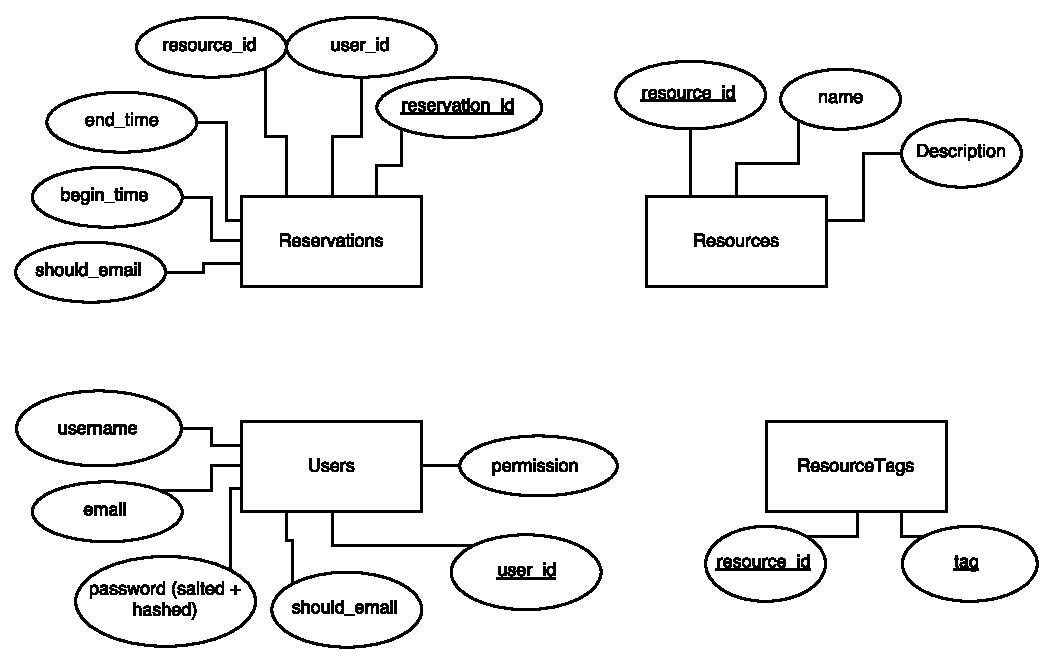
\includegraphics[width=6in]{Evolution1DB_cropped.pdf}

\end{document}